\thispagestyle{empty}
\tikz[remember picture,overlay] \node[inner sep=0pt,opacity=0.2] at 
(current page.center){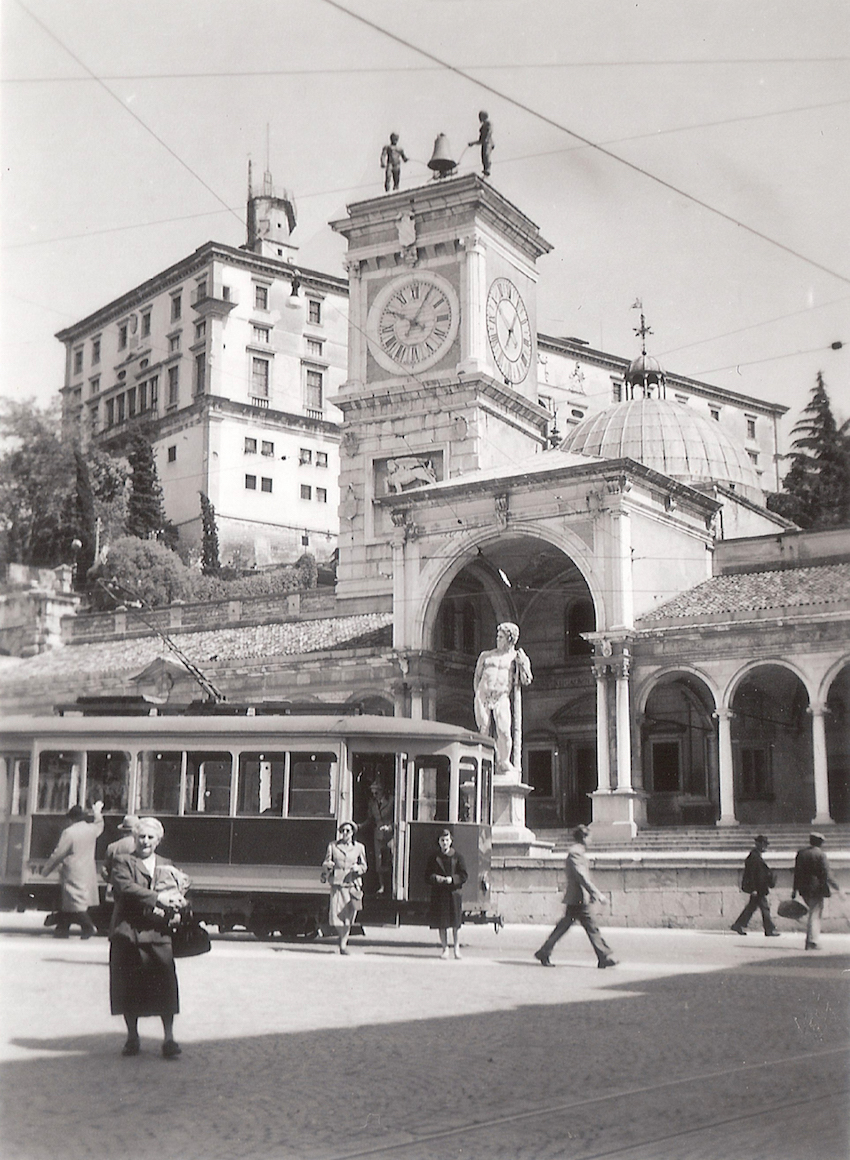
\includegraphics[width=\paperwidth,height=\paperheight
]{Gfx/piazza}};

\tikz[remember picture,overlay] \node[inner sep=0pt] at 
(current page.center){%inizio minipage
%
\begin{minipage}[c][0.8\paperheight][c]{0.8\paperwidth}

\begin{center}
\textsc{
{\huge Università degli Studi di Udine}
\bigskip 
\hrule
\bigskip
\begin{Large}
Dipartimento di Matematica, Informatica e Fisica\\\bigskip
Corso di Dottorato in\\ Informatica e Scienze Matematiche e Fisiche\\\bigskip
Ciclo XXXI
\end{Large}
}

\vfill

{\Huge \textsc{Model Checking:}}
\\ \vspace{0.3cm}
{\Huge \textsc{the Interval Way}}
\\ \vspace{1cm}
{\huge Tesi di Dottorato}

\vfill

\begin{Large}
\begin{flushleft}
Relatore \\ 
prof.\ Angelo MONTANARI\\\bigskip
Correlatore\\
prof.\ Adriano PERON
\end{flushleft}
\begin{flushright}
Dottorando \\
Alberto MOLINARI
\end{flushright}
\end{Large}
%
%\vfill
%
%\hrule
%\bigskip
%{\Large Anno Accademico 2018/2019}
\end{center}

\end{minipage}
};%fine minipage